%% ========================================================================
%%  JANUS-SR   Janus Speech Recognition Toolkit
%%             ------------------------------------------------------------
%%             Object: Description of basic decoding
%%             ------------------------------------------------------------
%%
%%  Author  :  Florian Metze & many others
%%  Module  :  basic.tex
%%  Date    :  $Id: basic.tex 2568 2004-11-09 19:54:57Z metze $
%%
%%  Remarks :  
%%
%% ========================================================================
%%
%%   $Log$
%%   Revision 1.4  2004/11/09 19:54:13  metze
%%   *** empty log message ***
%%
%%   Revision 1.3  2004/08/16 16:11:58  metze
%%   Additions for P014 by Florian
%%
%%   Revision 1.2  2003/08/14 11:19:02  fuegen
%%   Merged changes on branch jtk-01-01-15-fms (jaguar -> ibis-013)
%%
%%   Revision 1.1.2.12  2003/08/07 13:01:27  metze
%%   *** empty log message ***
%%
%%   Revision 1.1.2.11  2003/07/14 15:30:04  metze
%%   More complete version for V5.0 P013
%%
%%   Revision 1.1.2.10  2003/06/26 15:08:40  metze
%%   Initial changes for V5.0 P013
%%
%%   Revision 1.1.2.9  2002/11/21 16:16:29  metze
%%   Pre-P012
%%
%%   Revision 1.1.2.8  2002/10/28 17:28:20  soltau
%%   *** empty log message ***
%%
%%   Revision 1.1.2.7  2002/10/11 07:37:18  metze
%%   Corrected labels for lib2tex.tcl
%%
%%   Revision 1.1.2.6  2002/10/04 13:31:18  metze
%%   More docu
%%
%%   Revision 1.1.2.5  2002/08/27 16:19:27  metze
%%   New version of automatic generator.
%%
%%   Revision 1.1.2.4  2002/08/01 13:42:21  metze
%%   Fixes for clean documentation.
%%
%%   Revision 1.1.2.3  2002/07/31 13:10:27  metze
%%   *** empty log message ***
%%
%%   Revision 1.1.2.2  2002/07/30 13:10:25  metze
%%   *** empty log message ***
%%
%%   Revision 1.1.2.1  2002/05/28 14:12:31  metze
%%   Initial version of the Janus/ Ibis documentation
%%
%%
%% ========================================================================

\section{Basic Decoding} \label{ibis:basic}

This  section describes how to  setup Janus  to produce hypotheses and
lattices   from      ADC      data     using     the     \Jgloss{Ibis}
decoder. \Jindex{Decoding}  can also  be done using  Janus' three-pass
decoder, which is however not documented here.

\subsection{Module list}

You'll need the following modules  (most of these modules were already
introduced in the description of training procedures):

\begin{enumerate}

\item A  \Jref{module}{PhonesSet}, describing the  phones you  want to
use.   An      example    description  file      can   be   found   in
\Jref{file}{phonesSet}.

\item A  set   of  \Jref{module}{Tags}, containing the    tags  (phone
modifiers)  in  your  \Jref{module}{Dictionary}; typically  ``WB'' for
word boundaries   only. An example  description file  can  be found in
\Jref{file}{tags}.

\item A \Jref{module}{FeatureSet},  which  contains your ADC data  and
derived   features   (MCEP,    LDA,    ...).     You  normally     use
\Jref{file}{featAccess}   and \Jref{file}{featDesc}   to locate  and
process the ADC file.

\item A \Jref{module}{CodebookSet},   which  contains acoustic  models
(Gaussians).    An  example description    file     can be  found   in
\Jref{file}{codebookSet}. You'll also need a parameter file.

\item A \Jref{module}{DistribSet},  which contains the mixture weights
for the   Gaussians.  An example   description  file can  be found  in
\Jref{file}{distribSet}. You'll also need a parameter file.

\item A DistribTree, an instance of \Jref{module}{Tree}, which defines
which distribution   to use for  which  model.  An example description
file can be found in \Jref{file}{distribTree}.

\item    A      \Jref{module}{SenoneSet},  which   is    a      set of
(context-dependent) sub-phone model states.

\item A  \Jref{module}{TmSet}, which describes the allowed transitions
between states.  An example description  file can be found in
\Jref{file}{tmSet}.

\item A \Jref{module}{TopoSet}, containing the useable topologies.  An
example description file can be found in \Jref{file}{topoSet}.

\item A TopoTree.   This module of type  \Jref{module}{Tree} describes
which topologies to use for  which phones. An example description file
can be found in \Jref{file}{topoTree}.

\item A \Jref{module}{Dictionary}, see \Jref{file}{dictionary}.

\item A \Jref{module}{SVocab}, the search vocabulary. An example
file can be found in \Jref{file}{svocab}.

\item A \Jref{module}{LingKS}, a language model. The standard language
models (NGramLM) are in ARPABO format and can for example be generated
with the CLAUSI tools, the CMU-SLMT or the SRI toolkit.

\item A    \Jref{module}{DBase},    the Janus   database    module, is
optional. The standard scripts however  make use of the database.  For
an  example of how to   generate the DBase,  have  a look  at the file
\texttt{scripts/genDBase.tcl}.

\end{enumerate}

The object hierarchy for the Ibis decoder looks as follows:\\

\ifpdf
  \centerline{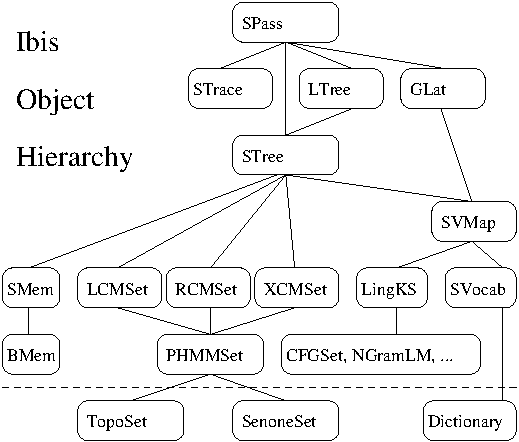
\includegraphics{hier}}
%  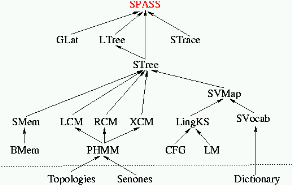
\includegraphics{ibis-hierarchy.png}
\else
  \centerline{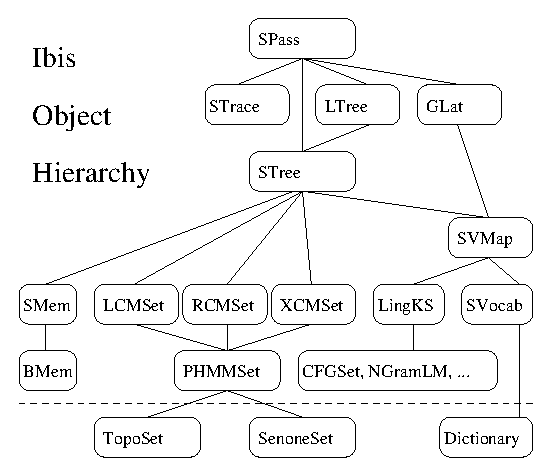
\psfig{file=hier.eps}}
\fi

The file \Jref{lib}{ibis.tcl} might save you a lot  of trouble.  Also,
consider looking at the example script \Jref{janus}{master.tcl}, which
in  turn  calls \Jref{janus}{test.tcl}.    This file will   start up a
standard decoder, which you  can then modify or re-configure according
to your   needs.   The initialization of  the    decoder can  be  done
automatically      by        calling      \Jref{proc}{ibisInit}   from
\Jref{lib}{ibis.tcl}  and  setting the values in \Jref{file}{desc.tcl}
correctly.

You can  also use  \Jref{proc}{lksInit} to set  up the  language model
independently from the decoder, this  makes it a  bit easier to handle
dumps generated by \Jref{module}{STree} \Jref{STree}{dump}  (remember,
when  you  read   a  dump,   you    cannot   load  the contents     of
\Jref{module}{Dictionary}  and \Jref{module}{SVocab}  and you can also
store the dump for the language model in the same file.


\subsection{Example decoding script}

A simple decoding script looks as follows:

\begin{verbatim}
source ../desc/desc.tcl

# ------------------------------------------------------
#  Init Modules
# ------------------------------------------------------

phonesSetInit   $SID
tagsInit        $SID
featureSetInit  $SID
codebookSetInit $SID
distribSetInit  $SID
distribTreeInit $SID -ptree ""
senoneSetInit   $SID  distribStream$SID
topoSetInit     $SID
ttreeInit       $SID
dictInit        $SID
trainInit       $SID
dbaseInit       $SID  [set ${SID}($dbaseName)]
ibisInit        $SID

# ---------------------------------
#   Here we go...
# ---------------------------------

while {[fgets $spkLst spk] != -1} {

    # --------------------------------------------------
    #   Loop over all utterances
    # --------------------------------------------------

    foreachSegment utt uttDB $spk {

        # preprocess audio data
        set uttInfo [dbaseUttInfo db$SID $spk $utt]
        featureSet$SID eval $uttInfo

        # run decoder
        spass$SID run

        # get hypothesis
        set hypo [spass$SID.stab trace]
        set text  [lrange $hypo 3 [expr [llength $hypo] -2]]
        puts "$utt: $text"

    }
}
\end{verbatim}
% $

The  DBase allows you to use  this double loop construct \texttt{while
fgets} and \texttt{foreachUtterance}  easily. The  outer loop (``while
fgets'') loops  over all speakers and allows  to  parallelize the work
over several machines,  by assigning  different speakers to  different
machines. The inner loop works  over all utterances of this particular
speaker.   Other loop constructions are   possible, of course.  Choose
whichever   is appropriate   for    your   needs.
% Have   a   look   at \Jref{janus}{fgets}.

Even     though   the   decoder  can    be    initialized  by  calling
\Jref{proc}{ibisInit}, you might want to have  a look at the following
sections on  decoder initialization and beam settings  to get a better
understanding  on   how things work,  although   the complexity can be
hidden      from    view     by     using   \Jref{proc}{lksInit}   and
\Jref{proc}{ibisInit}.

\subsection{Beam Settings}

The tuning   of beam  thresholds  to  speed   up the decoding  without
increasing search errors is dependent on  the task and the effectivity
of  the language    model  lookahead.   In  \cite{soltau:asru2001},  a
background about the decoding  technology can be found.  In principle,
there  are  three  thresholds to control   the  beam search.  The {\em
stateBeam} controls  the number   of  active states,  while the   {\em
wordBeam} controls the   number of active  word  ends.  The number  of
linguistically morphed instances, which depends on your language model
history,  is pruned  using  the {\em morphBeam}  threshold.  To reduce
high peaks in  memory consumption, a cutting  of active word  ends and
instances is  performed with {\em  transN} and  {\em morphN}.   For an
effective pruning, the following rules can be applied:

\begin{itemize}
\item $morphBeam$ $\ll$ $wordBeam$ $\ll$ $stateBeam$
\item $morphN$ $\ll$ $transN$ 
\end{itemize}

It should be noted that the language model weight has a high impact on
the   pruning  process.   That  means,  the  optimization  of  pruning
thresholds must    be done  with  respect   to  the   language   model
weights. Examples for the beam settings  for different tasks are given
here:

\begin{verbatim}
# read Broadcast News
spassX3 configure -stateBeam 130
spassX3 configure -wordBeam   90
spassX3 configure -morphBeam  80
spassX3 configure -transN 35 -morphN 8

# conversational telephony speech
spassX3 configure -stateBeam 195
spassX3 configure -wordBeam  135
spassX3 configure -morphBeam 120
spassX3 configure -transN 80 -morphN 20
\end{verbatim}

The  Ibis  decoder's  performance with  a  given set  of  acoustic and
language models   is   mainly governed by   the   beam settings. These
directly influence the search space and the tradeoff between speed and
accuracy.

If you  need faster recognition  time, there  are  two main techniques
implemented in JRTk to help  you achieve this goal: Gaussian Selection
(BBI)   reduces  the   number  of  Gaussians  evaluated   during score
computation  and   Phonetic Fast   Match (LookAhead)  prunes  unlikely
hypotheses away much earlier, therefore reducing the search space.

Also, Feature Space Adaptation   is a useful technique  that  improves
both speed and accuracy for a given system if you  have enough data to
adapt on. These techniques are described in the following sections.

\subsection{Gaussian Selection (BBI)}

Gaussian Selection using the Bucket-Box-Intersection algorithm
\cite{fritsch:icassp96} is the most popular speed-up algorithm for
Janus.   The script \texttt{createBBI.tcl} (\ref{janus:createBBI.tcl})
can be used to compute boxes for a given depth  and cut-off value. The
resulting description and parameter files can then be loaded into the
\Jref{module}{CodebookSet} using  \Jref{proc}{bbiSetInit}, as shown in
the script \texttt{test.tcl} (\ref{janus:test.tcl}).

Usually, you can achieve a speed-up by a factor of two with only minor
degradation in performance ($<$ 1\%).

\subsection{Phonetic Fast Match (LookAhead)}

A    Phonetic    Fast   Match      consists   of     an     additional
\Jref{module}{SenoneSet},   which is    based   on context-independent
codebooks. These are evaluated with a fixed  topology up to (normally)
5 frames ``in  the future''  and their  score is  added to the  normal
acoustic model score. Unlikely hypotheses  (``this does not look  like
an \texttt{/s/} in  the next 5 frames'') can  therefore be pruned away
much earlier, which  speeds up decoding  despite the overhead of extra
score computations.

An example script looks like this:

\begin{verbatim}
[...]

ibisInit        $SID -streeDump ../test6-b-6/streeC.gz                      \
                     -lmDesc    ../bigVocab/isip_ntp10+ch+cell+swb3.ibis.gz \
                     -lmType PhraseLM  -xcm 1

[...]

[FMatrix ldaLA]                  bload /project/ears2/X7/trainCI/ldaX7.bmat
[CodebookSet cbs featureSet$SID] read  /project/ears2/X7/desc/codebookSetLA
[DistribSet  dss cbs]            read  /project/ears2/X7/desc/distribSet

cbs load /project/ears2/X7/trainCI/Weights/4.cbs.gz
dss load /project/ears2/X7/trainCI/Weights/4.dss.gz

Tree dst phonesSet$SID:PHONES phonesSet$SID tags$SID dss
dst configure -padPhone @
dst read  /project/ears2/X7/desc/distribTreeLA

DistribStream str dss dst
SenoneSet     sns str -phones phonesSet$SID:PHONES -tags tags$SID

spass$SID fmatch sns
spass$SID configure -fastMatch 1.0

proc featureSetEvalLA {fes uttInfo} {
    global SID
    $fes matmul LDA-LA FEAT+ ldaLA -cut 42
}
FeatureSet method evalLA featureSetEvalLA  -text ""

[...]

while {[fgets $uttLst utt] >= 0} {

    [...]

    featureSet$SID eval   $uttInfo
    featureSet$SID evalLA $uttInfo

    [...]

    TIME START run $utt; spass$SID run; TIME STOP run $utt

    [...]
\end{verbatim}

You can   also   initialize a  LookAhead  system    by  specifying the
\Jref{ibisInit}{-fastMatch} option  to \Jref{proc}{ibisInit}. Be aware
that  the Fast  Match does not   have  any topology information.   You
therefore have to make sure you have models for all sub-phonetic units
in the distribution \Jref{module}{Tree}.  Typically you would specify
\texttt{ROOT-m} or \texttt{ROOT-b  ROOT-m} to the \Jref{SPass}{fmatch}
method  via the \texttt{-snTag}  option, which allows some flexibility
in which models to use for the  Fast Match. In some  cases it might be
necessary to manually  add \texttt{SIL-m} to the  \texttt{ROOT-b} part
of the distribution \Jref{module}{Tree}.

\subsection{Timing} \label{ibis:timing}

Speed-up methods  such as  the  ones just  discussed always  trade off
speed against  accuracy. How accuracy  can be measured is discussed in
section \ref{basic:scoring}, of  course JRTk also contains  mechanisms
to  estimate the  speed of  a process. The  relevant  script is called
\texttt{scripts/ana\_time.tcl} (see section \ref{janus:anatime.tcl}).

You'll need to define the following settings in your decoding (or any
other) script, to use \texttt{ana\_time.tcl}:

\begin{description}
\Jitem{... (CODE)} Some code
\Jitem{set ModulStatus(Timing) 1} to switch on timing analysis mode.
    If this variable is undefined or st to 0, nothing will happen.
\Jitem{... (CODE)} follows, no timing analysis
\Jitem{TIME START total \$utt} To start a block called ``total'' which
    you want to time for all utterances
\Jitem{... (CODE)} for ``total'' follows
\Jitem{TIME START run   \$utt} To start another block called ``run'', 
    it is also part of ``total''
\Jitem{... (CODE)} for ``run'' and ``total''
\Jitem{TIME STOP  run   \$utt} ``run'' ends here
\Jitem{... (CODE)} More ``total'' code
\Jitem{TIME STOP  total \$utt} ``total'' ends here, too
\Jitem{...(CODE)} Cleaning up
\Jitem{saveTIME "time.$[$pid$]$"} generates a file containing the 
    timing information, which can be used for further analysis
\Jitem{...} 
\end{description}

The  script   \texttt{scripts/test.tcl} contains   the necessary code,
although  it is switched  off by default.  Once  you ran a script with
these commands, you have two options:

\begin{enumerate}
\item Look at the output (the log-file). It will now contain lines such as
\begin{verbatim}
...
START total tobias_breyer.99 (1699.580000, 13.810000)
    featureSetISLcd ADCfile tobias_breyer.99 WARP 1.060
START run tobias_breyer.99 (1699.620000, 13.820000)
STOP run tobias_breyer.99 (1701.180000, 13.820000)
...
\end{verbatim}
  which tell you that decoding the utterance ``tobias\_breyer.99'' took
  1701.18-1699.62=1.56 seconds of CPU (user-) time.
\item If you have \texttt{time.$\ast$} files, you can use 
  \texttt{ana\_time.tcl} and generate a summary report by calling 
  \texttt{ana\_time.tcl} as follows in the test directory, i.e. the 
  directory in which you ran the test script and which contains the 
  \texttt{time.$\ast$} files:
  \begin{verbatim}
janus ~/janus/scripts/ana_time.tcl /project/njd/IslData/scoring/utts 5319.16
  \end{verbatim}
  The first parameter is the list of utterances to time. If you don't have
  it, it is normally very easy to generate this from the log-files or
  the data base. The second parameter is the total time of these utterances
  in seconds. Running this script should generate the following output: 
  \begin{verbatim}
ReadTime: time.16274
/project/njd/IslData/scoring/utts -> 831 utterances
duration        = 5319.16s
RTF run         : 0.29442806759
RTF total       : 0.318975176532
RTF warp        : 0.0174689236646
  \end{verbatim}
  The first line contains the name(s) of the time dump files read, the
  second  line the  number of  utterances  taken into account and  the
  third line the total time used. The next lines contain the real-time
  factors (xRTF) calculated for  the different blocks. This example is
  from decoding the IslSystem on a 3GHz P4 machine.
\end{enumerate}

The times reported by this method are  generated by the \texttt{times}
C-library function     and  returned  as     \texttt{tms\_utime}   and
\texttt{tms\_stime}. Be warned that the values you get will frequently
be meaningless on  SMP  machines and  if the  machine was  running two
processes (for a single-CPU system) or even swapping.

\subsection{Feature Space Adaptation (FSA)}

The ML adaptation technique described in \ref{janus:advanced} can also
be   applied  during decoding. In  this   case, you  simply compute an
adaptation  matrix  to transform the  features   to better match  your
models. The advantage in transforming the input features is of course,
that you don't have to touch the models, making  it possible to retain
BBI and Fast Match models.

Initialization of the necessary objects can be as simple as:

\begin{verbatim}
set sas signalAdapt${SID}
SignalAdapt $sas senoneSet$SID
$sas configure -topN 1 -shift 1.0
foreach ds [distribSet$SID] { $sas add $ds }
\end{verbatim}

Assuming you have created a \Jref{module}{Path} object containing your
current  hypothesis  and  your  codebooks  are  based  on the  ``LDA''
feature, the following code will accumulate sufficient statistics:

\begin{verbatim}
    # Feature space adaptation
    $sas clear     0
    $sas clearAccu 0
    $sas accu      path$SID 0
    $sas compute   10 0 0
    $sas adapt featureSet${SID}:LDA.data featureSet${SID}:LDA.data 0
\end{verbatim}

You can now decode again (without re-evaluating  the feature set). The
resulting  hypothesis should have a better   score than before and, on
average, the error rate will be lower.

It  is often a good idea   to only adapt the  features,  once you have
accumulated enough data (say 10 seconds of  speech). Assuming you have
more  utterances from  one  speaker or from  one  channel,  you can of
course accumulate the data over several utterances, compute the matrix
and re-decode. The  \Jref{module}{SignalAdapt} object can hold several
accumulators and  adaptation matrices  at the  same time.  It  is also
possible  to load and  save them.  Another idea is  to compute Viterbi
scores for several  adaptation matrices in order  to find the ``best''
one  and use it  for further adaptation. In   a demo system, you could
compute  in  advance  adaptation   matrices  for several   speakers or
channels and, during showtime, decode the first utterance once without
adaptation, pick the best adaptation matrix and  use if for subsequent
utterances, further adapting it to the current situation. This is
called ``delayed adaptation''.

%%% Local Variables: 
%%% mode: latex
%%% TeX-master: t
%%% End: 
